\scanpage{47}
% archive foliation: 46
% lines 1-5, upper-left diagram
\figure{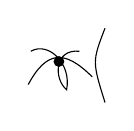
\begin{tikzpicture}[scale=.65]
\draw (-.55,.2) .. controls (-.2,.4) and (.25,-.05) .. (.15,-.55) .. controls (-.1,-.35) and (-.1,.25) .. (.4,.2);
\draw (-.6,-.45) .. controls (-.25,.2) and (.1,.25) .. (.65,-.3);
\fill (0,0) circle (3pt);
\draw (.9,.65) .. controls (.65,0) .. (.9,-.8);
\end{tikzpicture}}
\diagram{\begin{tikzcd}[row sep=large,column sep=large]
X_n=\unsure{\operatorname{Sp\hat ec}} k[x_n] \arrow[d] & \deleted{\unsure{x_n}}x_n^n=x_1 \\
X_1=\unsure{\operatorname{Sp\hat ec}} k[x_1=z] \arrow[d] & \left[\begin{array}{ccc}n&\vdots&n\end{array}\right] \\
X_0=\unsure{\operatorname{Sp\hat ec}} k[u] & \left[\begin{array}{ccc}2&2&\vdots\end{array}\right]
\end{tikzcd}}
\figure{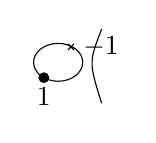
\begin{tikzpicture}[scale=.65]
\draw (0,0) ellipse (.48 and .37);\fill (-.28,-.3) circle (3pt);
\node[below] at (-.28,-.3) {$1$};\draw (.25,.3) ++(-.06,-.06)--++(.12,.12);\draw (.25,.3) ++(-.06,.06)--++(.12,-.12);\node[right] at (.3,.3) {$-1$};
\draw (.85,.65) .. controls (.6,0) .. (.85,-.8);
\end{tikzpicture}}
\[
u=\frac12-\frac14(z+z^{-1})
\]
% lines 2-4, upper-right
ramification au-dessus des \unsure{p\textsuperscript{ts}} $0,\infty$ (où la ramification est $n$)

\unsure{p\textsuperscript{ts}} de ramification en haut : $0,\infty$
% lines 5-9, upper-right
ramification au dessus de
\[
\begin{array}{ll}
0 & \deleted{\unsure{pas ramifié}\ (\unsure{p\textsuperscript{ts} au dessus}}\inserted{(z=1\ \text{ramification }2)}\\
1 & (z=-1,\ \text{ramification }2)\\
 & \deleted{\unsure{idem}}\\
\infty & (0\text{ et }\infty\ \text{ramification }1)
\end{array}
\]
% line 6, left
\[
D_\infty=(Z_{/2})\mathbin{\underset{\unsure{1/2}}{\cdot}}\mu_\infty
\]
% lines 10-14, middle diagrams
\diagram{\begin{tikzcd}[row sep=large,column sep=small]
0\ (n)\arrow[d]& &\infty\ \unsure{(n)}\arrow[d]&1\ (1)\arrow[d,"{n\ \text{fois}}"{description,draw,ellipse}]&\deleted{\unsure{-1|\infty}\ (1)}\arrow[d,draw=none,"{\deleted{\downarrow}}"{description}]&\text{$n$ pair}\\
0\ (1)\arrow[dr]&&\infty\ (1)\arrow[dl,dash]&1\ (2)\arrow[d]&-1\ \deleted{\unsure{0\ (2)}}\ (2)\arrow[d]&\\
&\infty&&0&1&
\end{tikzcd}}
\figure{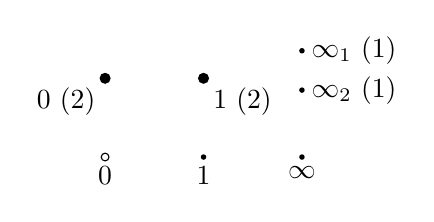
\begin{tikzpicture}[x=1.25cm,y=1cm]
\fill (0,0) circle (2pt);\node[below left] at (0,0) {$0\ (2)$};
\fill (1,0) circle (2pt);\node[below right] at (1,0) {$1\ (2)$};
\fill (2,.35) circle (1pt);\node[right] at (2,.35) {$\infty_1\ (1)$};
\fill (2,-.15) circle (1pt);\node[right] at (2,-.15) {$\infty_2\ (1)$};
\draw (0,-1) circle (1.4pt);\node[below] at (0,-1) {$0$};
\fill (1,-1) circle (1pt);\node[below] at (1,-1) {$1$};
\fill (2,-1) circle (1pt);\node[below] at (2,-1) {$\infty$};
\end{tikzpicture}}
% lines 15-17, lower graph
\figure{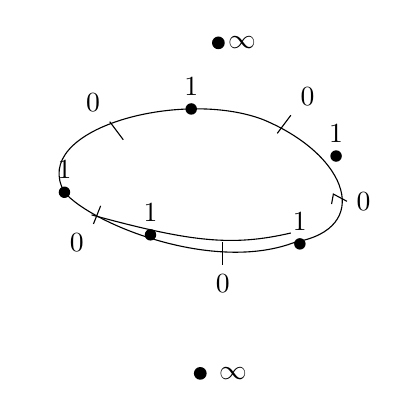
\begin{tikzpicture}[scale=1.15]
\fill (.2,1.65) circle (2pt);\node[right] at (.2,1.65) {$\infty$};
\draw (-1.5,0) .. controls (-1.9,.7) and (-.2,1.15) .. (.7,.8);
\draw (.7,.8) .. controls (1.65,.4) and (1.9,-.4) .. (1.05,-.55) .. controls (.15,-.9) and (-1.2,-.35) .. (-1.5,0);
\draw (-1.2,-.25) .. controls (-.1,-.55) and (.35,-.6) .. (1,-.45);
\foreach \x/\y/\lab in {-1.5/0/1,-.1/.92/1,1.5/.4/1,1.1/-.57/1,-.55/-.47/1}{\fill (\x,\y) circle (1.8pt);\node[above] at (\x,\y+.04) {$\lab$};}
\draw (-1,.78)--(-.85,.58);\node[above left] at (-1,.78) {$0$};
\draw (.85,.65)--(1,.85);\node[above right] at (1,.85) {$0$};
\draw (1.62,-.1)--(1.47,-.02)--(1.45,-.13);\node[right] at (1.62,-.1) {$0$};
\draw (.25,-.55)--(.25,-.8);\node[below] at (.25,-.8) {$0$};
\draw (-1.1,-.15)--(-1.18,-.35);\node[below left] at (-1.18,-.35) {$0$};
\fill (0,-2) circle (2pt);\node[right] at (.1,-2) {$\infty$};
\end{tikzpicture}}
% lines 18-19, inverted printed label
\begin{tabular}{l}
MR LE PROFESSEUR GROTHENDIECK A.\\
MATHEMATIQUES\qquad 5
\end{tabular}
